\section{Overlay Mesh}

\subsection{Self–Optimisation}
Nodes in the Mitosis network constantly try to improve their own connections. As discussed in \vref{sec:design-peers}, this should lead to a more stable system in general.

In this experiment, the positioning of peers in relation to the router is measured. Running a simulation with $n=200$ nodes for $t=1000$ ticks, the distance from each peer to the router is put in relation to the simulated network configuration of the peer. In this scenario, connection latency is configured to a random value in the range of $0.125<l<0.5$ ticks, connection establishment delay falls in the range of $0.1<1.0$ ticks and the drop probability for messages on the unreliable channel \cref{sec:mit-connections} is set to $0.0<s<5.0$ percent. For simplicity, every peer is assigned values within these ranges at instantiation and those values remain static throughout the simulation.

As peers strive to acquire connections to peers with a good router link quality and a good connection quality, the hypothesis is that peers with good connection qualities will \say{bubble} towards the router. For verification, at the end of the scenario, every peer reports its network configuration parameters along with its distance to the router node. Distances are calculated in hops using the Dijkstra algorithm and treating the mesh as an undirected and unweighted graph.
\cref{fig:connection-quality-per-distance} shows the histogram of network quality settings binned by router distance. For comparability, the settings are normalised to percentages corresponding to the aforementioned ranges, with higher percentages representing the \textit{better} end of the range.

\begin{figure}[htb!]
\centering
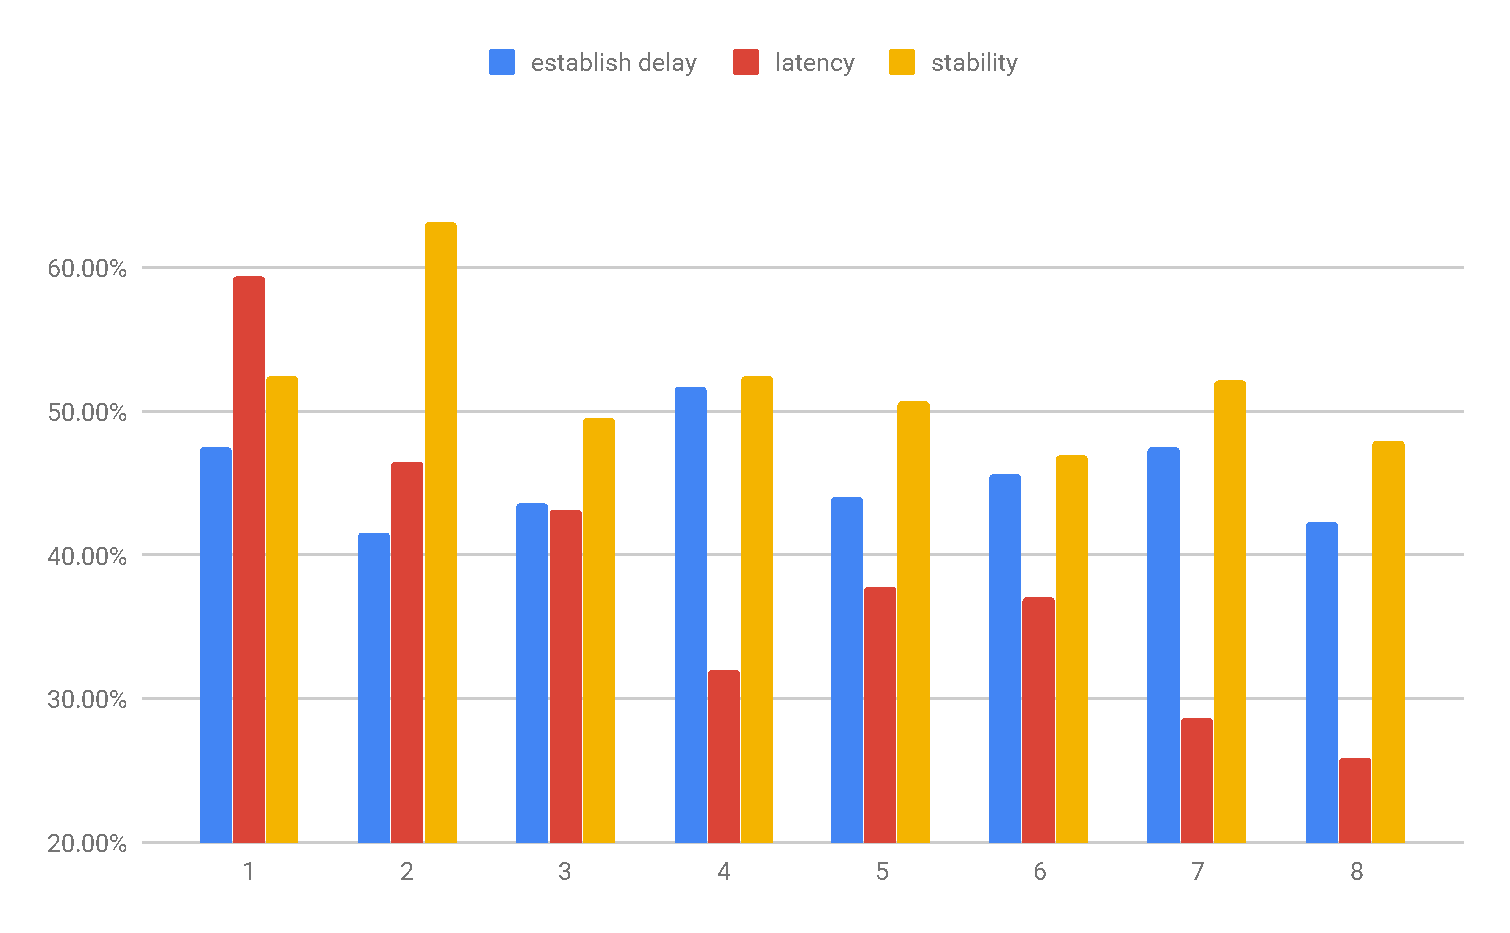
\includegraphics[width=1.0\textwidth]{graphics/analysis/connection-quality-per-distance.pdf}
\caption{Network quality of nodes in relation to their router distance}
\label{fig:connection-quality-per-distance}
\end{figure}

As to be expected, establishment delays do not show a dependency on router distance. Nodes only begin metering the quality of a connection after it has been opened. In fact, this is a desirable behaviour, since \gls{webrtc} connections can take a while to generate \gls{ice} candidates and to establish. Yet, the grade of the \gls{webrtc} connection does not relate to how long the establishment took.

The distribution of average connection latency per router distance is in line with the hypothesis. Nodes with below average latency (circa $l<0.27$) have acquired direct connections to the \router node, while nodes with only half as responsive connections have been pushed outwards to be leaf nodes.

The stability for the unreliable channel shows a distribution proximate to the latency, but not as clear. Nodes with low message drop probabilities, accumulate to distance levels one and two, yet the falloff is not as distinctive. This can be explained by looking back at the utilisation of the unreliable channel in \vref{par:webrtc-data-measure-quality}: The \gls{tq} of the connection meter is intended to access the duplexity of the connection and the responsiveness of the peer. However, in the simulation, the drop probability is applied to both incoming and outgoing messages.

\subsection{Ingress Rates}

For a \gls{p2p} network to reach its potential scale, not only does it need to retain a high number of peers, it needs to take them in at a high rate. In real–world applications users can join and exit in unpredictable bursts, which can cause queues at the entry point or leaf gaps in the middle of the mesh.

The Mitosis mesh design envisions a clustered landscape \cref{par:scaling-cluster}, where peers are associated to a router by a signal server. These router peers are the only way into the mesh and naturally have a maximum rate at which they can absorb new peers and forward them into the mesh. In real–world applications, the ingress rate would depend on the network and computing capabilities of the router peer, as well as the size and structure of its mesh. For the purposes of identifying the ingress rate under optimal conditions, these factors are intentionally left untouched.

A new mesh is created by spawning nodes at a static rate and metering how fast they are connected to at least one peer of the mesh (excluding the signal server). Spawn rates were set to $3.2<r<12.5$, while the maximum node amount was set to $n=100$. \Vref{fig:ingress-rates} shows three distinct runs of this experiment, where the dotted lines show the number of spawned nodes and the solid line shows the number of successfully absorbed nodes. A clear disparity can be seen between the lines for $r=12.5$. This hints towards multiple nodes queuing up at the entry point. For $r=3.2$, the network's ingress seems to lag only a few nodes behind the spawn rate. These lines run in parallel, indicating that apart from nodes currently in transition, no queue is forming. So, for the default configuration of the \textit{Mitosis} core library and in a flawless network setting, this would be the optimal value.

\begin{figure}[htb!]
\centering
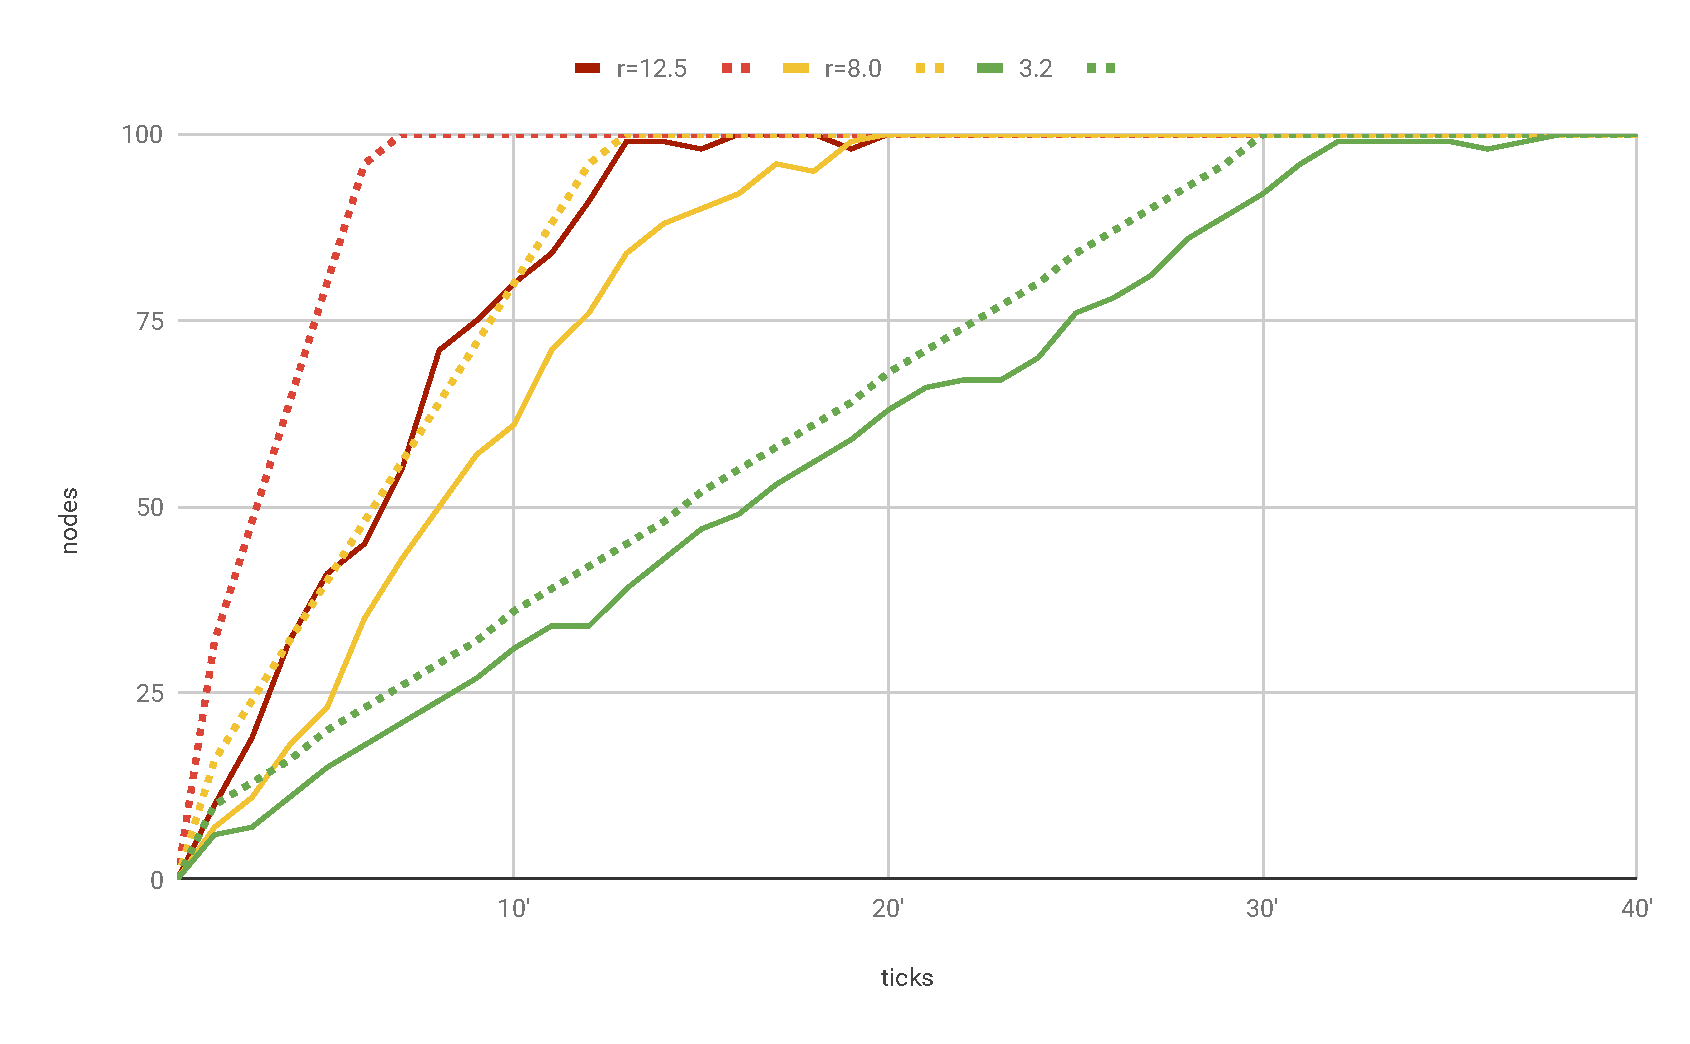
\includegraphics[width=1.0\textwidth]{graphics/analysis/ingress-final.pdf}
\caption{Ingress rates in relation to join rates in nodes per tick}
\label{fig:ingress-rates}
\end{figure}

This experiment shows how an important factor of mesh scalability can be measured. The actual numerical outcome, however, is to be taken with a grain of salt. Instead, signal servers would need to detect this rate during runtime and adjust the number of clusters according to demand.


\subsection{Connection Limits}

One other important facet of the mesh configuration, is the range connection goal and maximum connection limit as introduced by \vref{sec:design-optimising}. These influence the mesh density and rigidity and help it take on more peers and better recover from connection loss. In this experimental run, the simulation is started goal range configurations from $g_{min}=1$ to $g_{max}=8$ with a range width of $g_{max}-g_{min}=2$. The maximum connection limit is set to $m=(g_{min}+g_{max})/2$. The node join rate is kept at a low value of $r=1$ for $t=500$ ticks and network conditions remain at stable settings.

The prediction is, that low connection limits will cause the network's connectedness to suffer but higher connection goals will bring proportionally more traffic overhead.
To verify this predicted behaviour of the mesh implementation, the total mesh size is measured in peers and the total network traffic per tick is calculated.
The mesh size is calculated by finding all \glspl{scc} in the graph and counting all nodes in the largest component. The network traffic is aggregated per tick across nodes by the simulator's message delivery system.

\Vref{fig:connection-limits-largest-component} shows the node count of the largest mesh component, when spawning a new cluster with different connection limits. It is easily visible, how a goal of $g\leq4$ causes the mesh to fail at taking in peers at a stable rate and growing past a size of $n\approx100$. The $3 \leq g \leq 5, m=8$ configuration, also shows one incident of unintentional mesh separation. All higher connection limits are able to gain and maintain their mesh size proportionally to the spawn rate.

\begin{figure}[htb!]
\centering
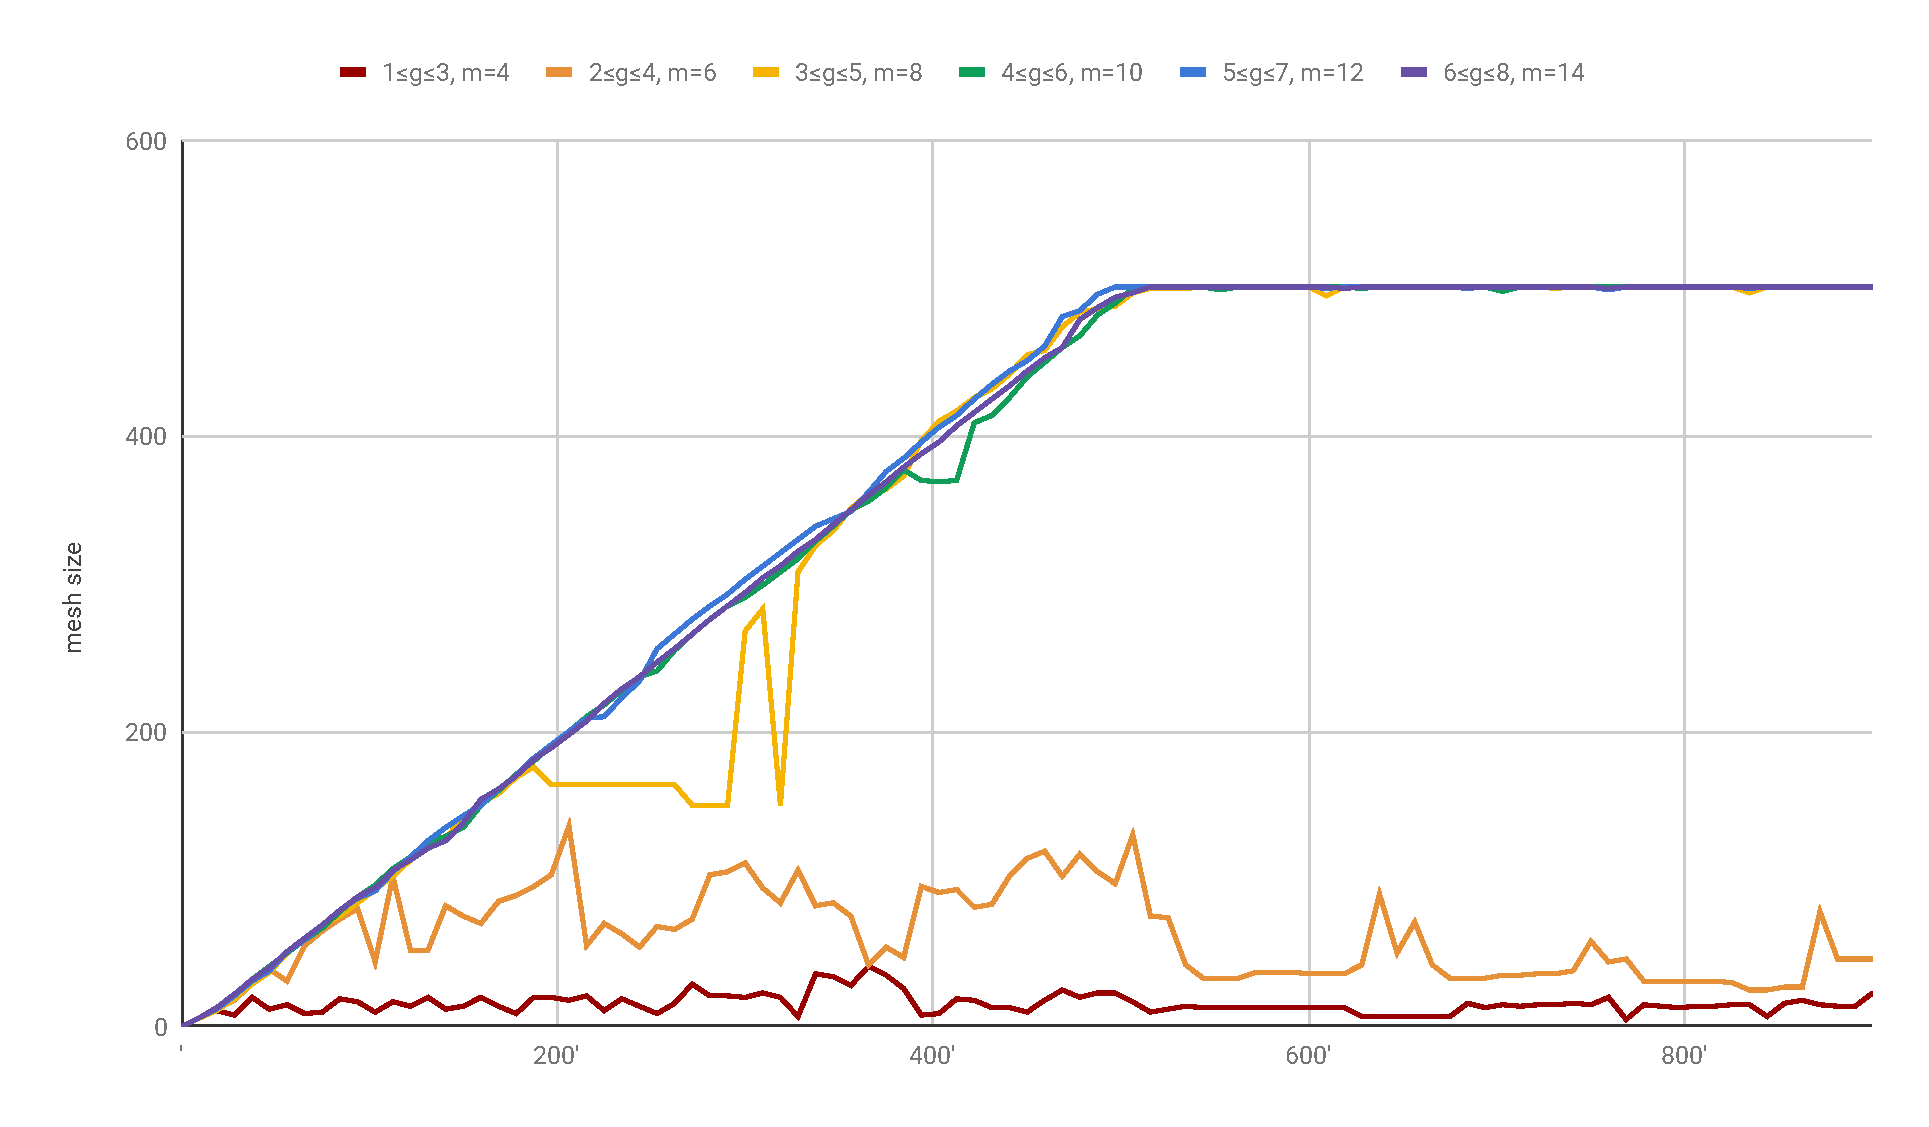
\includegraphics[width=1.0\textwidth]{graphics/analysis/connection-limit-largest-component.pdf}
\caption{Mesh size in nodes in relation to connection limits}
\label{fig:connection-limits-largest-component}
\end{figure}

\Vref{fig:connection-limits-total-io} details the growth in traffic the network has to handle collectively per tick in megabytes. This diagram paints the opposite picture, as configurations with lower connection limits cause significantly less traffic overhead. The extra traffic is due to more Ping/Pong and \peerUpdate messages being sent to keep the network alive and peers informed.

However, total traffic is just one indicator, how higher connection limits do not imply a more performant network. With more connections, nodes will take on more neighbours and their routing table will grow exponentially. Routing will therefore become more complex and finding the best path to the router or the best peering candidate more ambiguous.

\begin{figure}[htb!]
\centering
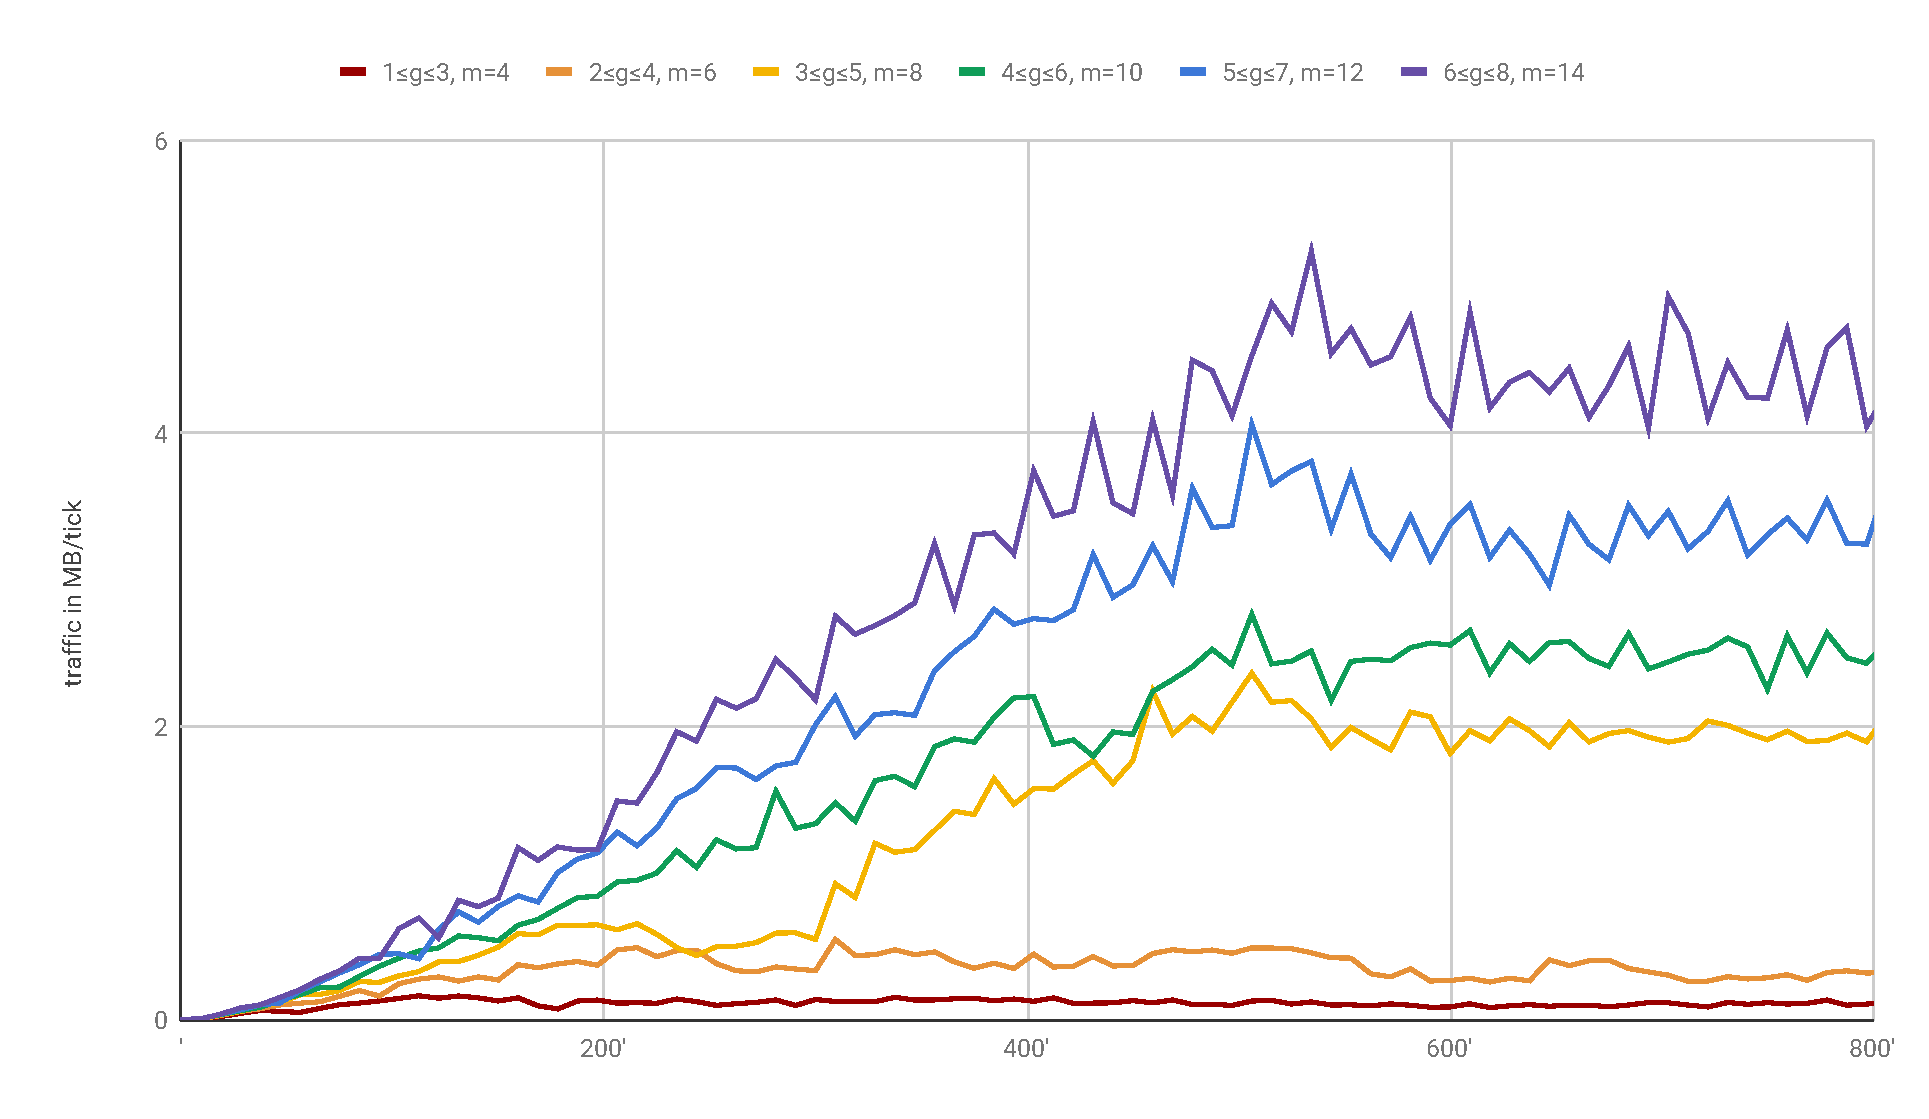
\includegraphics[width=1.0\textwidth]{graphics/analysis/connection-limit-total-io.pdf}
\caption{Network–wide traffic per tick in relation to connection limits}
\label{fig:connection-limits-total-io}
\end{figure}
